\documentclass[a4paper,12pt]{article}

\usepackage{natbib}
\usepackage{times}
\usepackage{graphicx,epsfig}
\usepackage[leftcaption]{sidecap}
\usepackage{subfigure} % figures can have sub chunks
\usepackage{geometry} % this maxes page usage, making the below unnecessary
\textwidth = 6.75in
\oddsidemargin = -0.25in
\textheight = 10in
\topmargin = -0.5in
\usepackage{fancyhdr}
\pagestyle{fancy}
\lhead{{\it Alan Lau}}
\chead{Wall Following LEGO Robots}
\rhead{Coursework 1}
\lfoot{}
\cfoot{\thepage}
\rfoot{}
\usepackage[T1]{fontenc}
\usepackage{multirow}
\usepackage{multicol}
\usepackage{array}
\usepackage{caption}
\usepackage{hyperref}
\usepackage{graphicx}
\graphicspath{ {images/} }

\usepackage{calc}
\setlength{\parskip}{6pt}
\setlength{\parindent}{0pt}
% \addtolength{\hoffset}{0.5cm}
% \addtolength{\textwidth}{0.5cm}

% set section depth
\setcounter{tocdepth}{4}
\setcounter{secnumdepth}{5}

\newcommand{\goodgap}{%
 \hspace{\subfigtopskip}%
 \hspace{\subfigbottomskip}}

\title{Coursework 1:  Wall Following with a LEGO Robot}
\author{Alan Lau}


\begin{document}
\maketitle

\section{Introduction}
We created a LEGO robot capable of navigating around obstacles along a wallside. During the development of the robot, we came up with the following hypothesis:

\begin{center}
    "There is an optimal combination of parameters that yields the fastest time in completing a pre-set course with obstacles for a reactive robot." 
\end{center}

Our aim is to explore how important prior knowledge impacts the success of a robot, and attempting to finding a correlation between these parameters so that we can obtain the best combination of parameters to successfully navigate through an obstacle-filled course.

Our approach centres with the idea of reactivity as described by \cite{brooks1991}. We focus our efforts in making our robot `generic', in the sense that our robot should handle a dynamic environment that it has not seen before, through sensing its surrounding, rather than hard-coding its behaviour around one specific course. Having said that, prior information is key. One requires the facility to rotate and move forward in order to perform navigation. By varying the speed and prior information. 

Our robot uses a sonar sensor and two touch sensors in order to support the reactive nature of its operation. The sonar sensor (`head') is attached to a motor which enables a 180-degree rotation (looking forward, to the right and to the left), and is mounted at a high position to capture big obstacles. The touch sensors (`bumper') are in a lower position to detect low-lying obstacles and collisions. 

% - hypothesis (what you tried to do)
% - motivation (why you have done that)
% - brief background for arguments
% - cite papers for motivation (e.g. Brooks 1991)
% - present a single hypothesis you tested on your completed robot about how to improve its intelligence

\section{Approach}
Simon Elvin (sje29) and I worked throughout the development of the robot. We pair programmed our robot in order to create the set of logic required to perform the appropriate actions as we desired. We also discussed, finalised the design and built our robot together. We also defined the conditions and parameters we are experimenting on, and jointly performed the experiments. However, the interpretation of the results is my own work.

First, we define some settings for our experiments. We ran our experiments using the `natural' course found in the MSc laboratory, as shown in \autoref{fig:course}. We belive this is a representative course for the purpose of our tests, as it contains both obvious angles, such as the ones around the black cabinet, and more challenging angles, such as those around the red cabinets and the bin in the diagram.

Also, we define `success' as being able to complete the course by going from the starting point to the end point. There are exceptions to the rule. For instance, in the unlikely event for the robot to reach the end



During our experiment, we recorded the number of collisions and the number of corners it missed or did not follow closely for further information. In the unlikely event that the robot

We view that colliding into the wall is bad, as an intelligent robot should be able to navigate smoothly around obstacles.

In our experiment, we altered the speed of the motors attached to the wheels, minimum distance between an obstacle and the robot, 

% Through the development of the robot, we incrementally increased its intelligence by focusing on reacting to the distance readings from the sonar sensor than the touch sensors.

% On top of the head movements, the actions that the robot can do include going forward, going backward and altering the motor speed and rotating to a specific angle. The combination of these actions form different behaviours of the robot. For instance, when the robot collides into the wall, it would go backwards for 1 second and then rotating by 45 degrees in the opposite direction of the identified wallside. 

% To enable the robot to reactively interact with any given indoor environment, the robot is programmed with 3 states and 6 commands, as listed in \autoref{tab:states-commands}. Each command in each state gives the robot a different behaviour. For instance, if the robot is in the state \texttt{FOLLOWING\_WALL} and has the command \texttt{TOO\_CLOSE}, it will perform a \texttt{smoothTurn} to try to rectify the fact that the robot is being too close to the wall by moving slowly away from the wall, as opposed to sharp turn.


% - describe in detail what exactly we have done 
    % - e.g. experiements set up to determine in what conditions you could make better results (replicability) (cite paper)
% - who I partnered with and how much we worked together
% - questions
    % - contrasting the addition of extra control algorithms
    % - changing the physical shape of the robot
    % - trying different target sonar readings for maintaining a particular distance
    % - circuit time, success rate
% - capture, describe the things that makes a difference in performance
% - consider chagning variables - battery, daylight, proximity to other sonar-using robots to explain strange behaviour


\section{Results}
% - describes the outcome - factual descriptions (qualitative, quantitative)
    % - significance testing & standard deviation - e.g. avg speed around a circuit in two conditions
% - video to prove the conditions lead to different results
% - precise, factual results only - info to be described in approach
% - an insightful comment about one or more cited papers
% supported by evidence from your experience might get you these extra
% marks
% - so might a particularly accurate and replicable account of
% your approach and results


\section{Discussion}

% - include speculation
% - discuss how results address the questions described in intro
% - how restuls imply about your own worka and AI or robotics in general
% - suggest other experiments that might give other insights
% - can be long with comparisons with papers 


\section{Conclusion}
% - on paragraph
% - restate what we tried to do and the outcome
% - results in light of the intro

\newpage
\bibliographystyle{apalike}
\bibliography{biblio}

\appendix
\section{Tables and Graphs}

%%%%%%%%%%%%%%%%%%% States-commands
{\renewcommand{\arraystretch}{1.3}%
\parbox{\linewidth} {
    \centering
  \begin{tabular}{|m{0.15\textwidth}|m{0.22\textwidth}|m{0.22\textwidth}|m{0.22\textwidth}|}
        \hline

%%%%%%%% States
        %\multirow{3}{*}{%}
    \textbf{States}
      & \texttt{FINDING\_WALL} & \texttt{FOLLOWING\_WALL} & \texttt{LOOKING\_FORWARD}
    \\ \hline
%%%%%%%% States 

%%%%%%%% Commands
    \multirow{6}{*}{\textbf{Commands}}
      & \multicolumn{3}{c|}{\texttt{TOO\_CLOSE}} 
      \\ %\cline{2-4}

      & \multicolumn{3}{c|}{\texttt{TOO\_FAR}} 
      \\ %\cline{2-4}

      & \multicolumn{3}{c|}{\texttt{IN\_RANGE\_FAR}} 
      \\ %\cline{2-4}

      & \multicolumn{3}{c|}{\texttt{IN\_RANGE\_CLOSE}} 
      \\ %\cline{2-4}

      & \multicolumn{3}{c|}{\texttt{INTERVAL\_REACHED}} 
      \\ %\cline{2-4}

      & \multicolumn{3}{c|}{\texttt{TOUCH\_CONTACT}} 
      \\ \hline
%%%%%%%% Commands

    \end{tabular}
\captionof{table}{\textit{States and commands used by the robot.}}
\label{tab:states-commands}
}
%%%%%%%%%%%%%%%%%%%%%%%

% FIG - methodology
\begin{figure}[h]
    \centering
    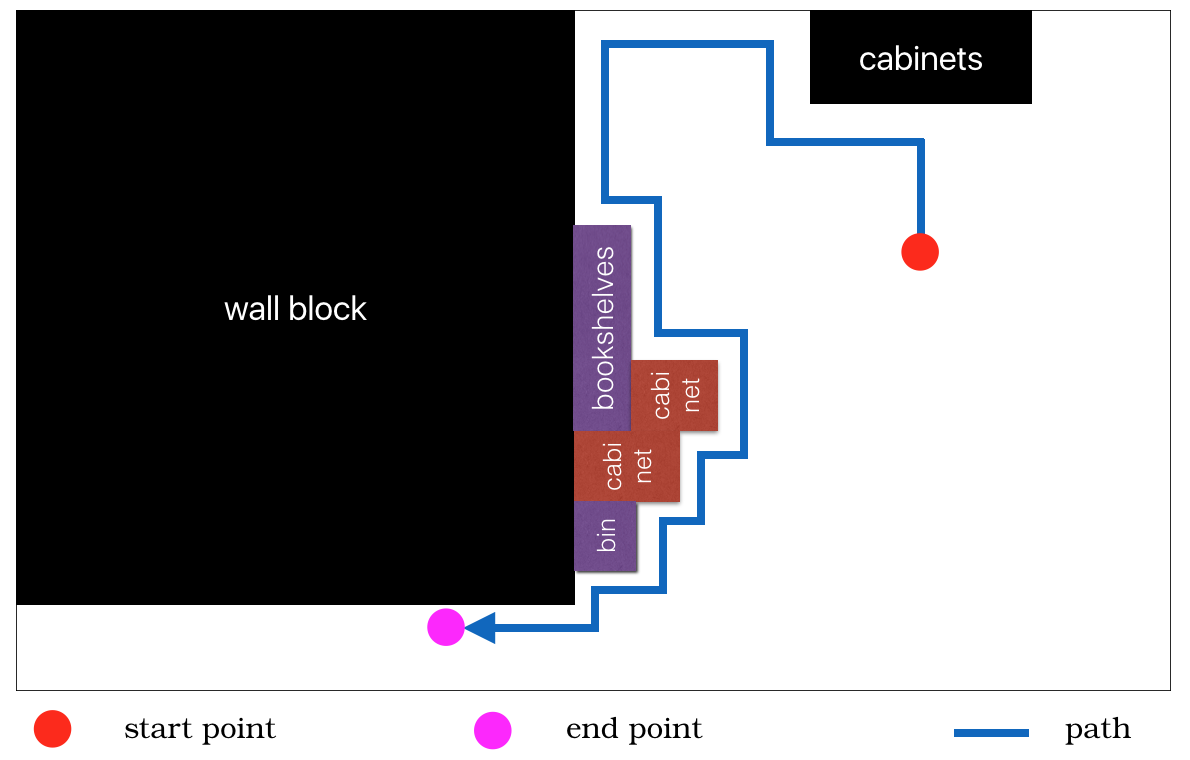
\includegraphics[width=0.9\textwidth]{path}
    \caption{\textit{A bird's-eye view of the course setup used to develop and test the robot against our hypothesis.}}
    \label{fig:course}
\end{figure}

\end{document}
